\documentclass[../ECE459FinalProjectReport.tex]{subfiles}

\begin{document}
\chapter{Methodology}
This chapter presents the methodology employed in the project using Python 3. The simulations were executed within the Jupyter Notebook environment, leveraging essential packages for numerical computation, signal analysis, and plotting, namely \verb|numpy|, \verb|scipy|, and \verb|matplotlib|.

\section{Choice of Message Signal}

Two distinct message signals were selected for thorough investigation in this project:
\begin{enumerate}
    \item The multi-tone sinusoidal signal $m_1 (t) = A_1\cos(2\pi f_1 t + \phi_1) + A_2 \cos(2\pi f_2 t + \phi_2)$.
    \item The TTS-generated male voice recording.
\end{enumerate}

The first signal, a multi-tone sinusoidal waveform, was chosen for its simplicity as a periodic function and its unique attributes as a linear combination of two sinusoidal functions. This particular choice facilitates the observation of distortion induced by noise, given the relatively straightforward frequency spectra of sinusoidal functions. On the other hand, the utilization of a TTS-generated male voice recording introduces a more realistic scenario, allowing the team to experiment with the designed communication system in a practical context.

\section{AM Simulation}
\subsection{Envelope Modulation}

The modulation of a message signal, denoted as $m(t)$, can be achieved through envelope modulation, represented by the equation:
\begin{equation}
    s(t) = A_c [1 + k_a m(t)] \cos (2\pi f_c t + \phi)
\end{equation}
where $\phi$ is the phase delay of the local oscillator. In this project, we pick $\phi = 0$ for simplicity.

In this expression, $k_a$ denotes the modulation sensitivity, $A_c$ corresponds to the amplitude of the carrier wave, and $f_c$ represents the frequency of the carrier wave. It is imperative to ensure that the carrier wave frequency $f_c$ significantly surpasses the highest frequency component, denoted as $W$, of the message signal $m(t)$ to prevent aliasing. This condition can be expressed as $f_c \gg W$. Moreover, the choice of the modulation sensitivity, $k_a$, needs to adhere to the constraint:
\begin{equation}
    \left| k_a m(t) \right| < 1, \quad \text{for all }t.
\end{equation}

This condition is crucial to prevent envelope distortion, as outlined by \textcite[pp. 101-102]{haykinIntroductionAnalogDigital2007}.

The implementation of amplitude modulation (AM) can be illustrated through the block diagram depicted in Figure \ref{fig:env-mod}.
\begin{figure}[b]
    \centering
    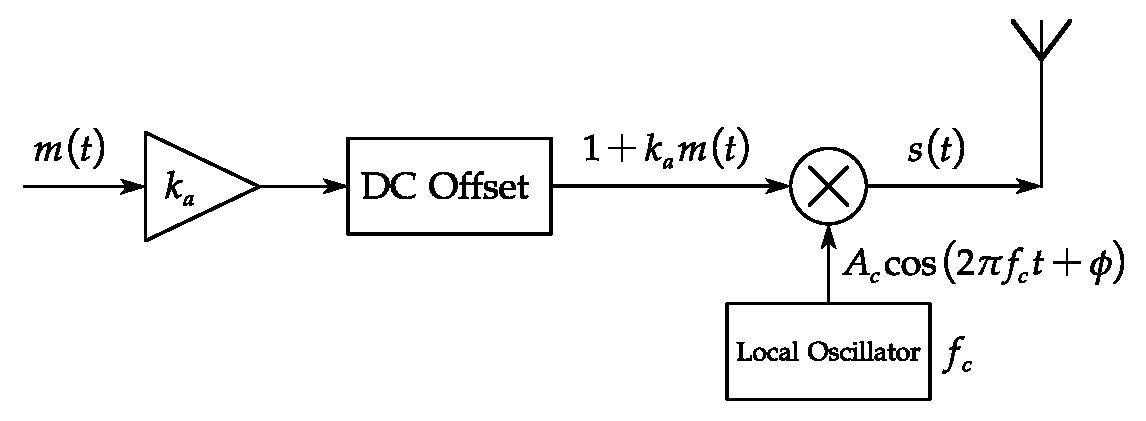
\includegraphics[scale=0.7]{plots/env_mod.pdf}
    \caption{Block diagram illustrating the process of envelope modulation.}
    \label{fig:env-mod}
\end{figure}

\subsection{Envelope Detection}
Diverging from coherent detection, envelope detection dispenses with the necessity of multiplying the received signal by the carrier wave. Instead, the received signal undergoes filtration by a Band Pass Filter (BPF) to eliminate noise beyond the desired bandwidth, and subsequently, an envelope detector facilitates the recovery of the message signal. This procedural sequence is depicted in Figure \ref{fig:env-demod}.

In physical circuitry, the envelope detector typically comprises a diode and an LPF \cite{AnalogCommunicationAM}. However, in Python, this functionality is realized through a Hilbert transform process \cite{ulrichEnvelopeCalculationHilbert2006, XiXiaoShengPythonTiQuXinHaoDeBaoLuoGet2023}.

Consider a single-tone sinusoidal signal with frequency $f_m$ modulated by a carrier wave with frequency $f_c$. The modulated wave, denoted as $g(t)$, is expressed as
\begin{equation}
    g(t) = \sin(2\pi f_c t)\sin(2\pi f_m t)
\end{equation}
where $f_c\gg f_m$. By trigonometric identity, $g(t)$ can be alternatively expressed as
\begin{equation}
    g(t)=-\frac{1}{2}\{\cos\mathrm[2\pi (f_c+f_m)t]-\cos[2\pi (f_c-f_m)t]\}.
\end{equation}

The Hilbert transform introduces a $-\frac{\pi}{2}$ to the phase of the signal, which yields
\begin{equation}
    \begin{aligned}
        \tilde{g}(t)&=-\frac{1}{2}\left\lbrace\cos\left[2\pi (f_c+f_m)t - \frac{\pi}{2}\right]-\cos\left[2\pi (f_c-f_m)t - \frac{\pi}{2}\right]\right\rbrace\\
        &=-\frac{1}{2}\left\{ \sin \left( 2\pi f_ct-\frac{\pi}{2} \right) \sin \left( 2\pi f_mt \right) \right\} \\
                    &=-\frac{1}{2}\cos \left( 2\pi f_ct \right) \sin \left( 2\pi f_mt \right) 
    \end{aligned}
\end{equation}

The analytic signal of $g(t)$, denoted as $\aleph\{g(t)\}$, can be expressed as a combination of $g(t)$ and its Hilbert transform $\tilde{g}(t)$, which is
\begin{equation}
    \aleph\{g(t)\} = g(t) + j\tilde{g}(t) = \sin(2\pi f_c t)\sin(2\pi f_m t) - j\cos(2\pi f_c t)\sin(2\pi f_m t).
\end{equation}

The magnitude of the analytic signal can be calculated by
\begin{equation}
    \left| \aleph\{g(t)\}\right| = \sqrt{\aleph\{g(t)\}\aleph^*\{g(t)\}} = \left| \sin(2\pi f_m t)\right|
\end{equation}
which precisely equals to the original $g(t)$.

Thus, the envelope of an envelope-modulated signal can be derived by calculating the magnitude of the Hilbert transform of the signal. This methodology is applied by the team in the project.

\begin{figure}[htb]
    \centering
    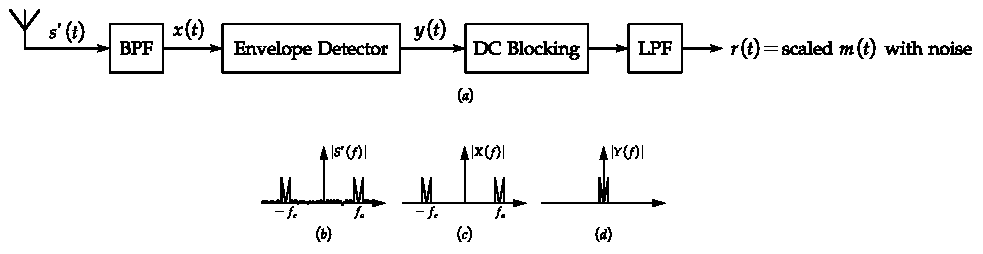
\includegraphics[width=.9\linewidth]{plots/env-demod.pdf}
    \caption{Block diagram illustrating the process of envelope demodulation.}
    \label{fig:env-demod}
\end{figure}

\subsection{SNR Calculation and Measurement}
~
\section{FM Simulation}
\subsection{Narrow-Band FM Modulation}
~
\subsection{Narrow-Band FM Demodulation}
~
\subsection{SNR Calculation and Measurement}
~
\section{Filter Design}
\subsection{Ideal Filters}
% 讲LPF和BPF的TF,然后引出为什么ideal filter无法实现,再引出butterworth
~
\subsection{Butterworth Filter in Python}

Both Amplitude Modulation (AM) and Frequency Modulation (FM) communication systems necessitate the incorporation of filters. In practical scenarios, however, the realization of ideal filters poses inherent challenges. Nevertheless, the Butterworth Filter exhibits characteristics closely approximating those of an ideal filter. Figures \ref{fig:butter-lpf} and \ref{fig:butter-bpf} depict the frequency responses of Butterworth Low Pass Filter (LPF) and Band Pass Filter (BPF) with varying orders, illustrating that an increased order ($n$) results in a more pronounced roll-off slope. As expounded by \cite{storrButterworthFilterDesign2013, kudekiAnalogSignalsSystems2009}, a Butterworth Low Pass Filter manifests a maximally flat frequency response within its passband, swiftly attenuating beyond the cut-off frequency. This advantageous attribute empowers the design of filters with minimal distortion, albeit at the expense of an indeterminate phase delay induced by the inherent properties of Infinite Impulse Response (IIR) filters.

In the digital realm, Python facilitates the implementation of filters as digital IIR/FIR filters, with each filter in the $z$-domain expressed as the quotient of two polynomials:
\begin{equation}
H_{\text{filter}}(z) = \frac{\sum_{p=0}^{n}{a_pz^{-p}}}{\sum_{q=0}^{n}{b_qz^{-q}}}
\end{equation}

The response of the filter is uniquely determined by coefficients $a_i$ and $b_j$ ($0 \leq i, j \leq n$), where these coefficients can be computed using the \verb|scipy.signal.butter()| function, as detailed by \cite{thescipycommunityScipySignalButter, thescipycommunityScipySignalFiltfilt, thescipycommunityScipySignalLfilter}. A practical instantiation of an IIR filter is exemplified below:
\begin{lstlisting}[language=python]
# Generate an 8-order 40 Hz to 80 Hz IIR BPF, sample rate = fs
b, a = butter(N=8, [40, 80], btype='band', fs=fs)
# Apply the filter to the message signal
filtered_signal = filtfilt(b, a, message)
\end{lstlisting}

Figures \ref{fig:butter-lpf} and \ref{fig:butter-bpf} showcase the frequency response of a Butterworth LPF and BPF, respectively, each featuring a cut-off frequency of $\omega_c = \SI{100}{\radian\per\s}$. The black dashed line denotes the \SI{-3}{\dB} amplitude.

\begin{figure}[htb]
    \centering
    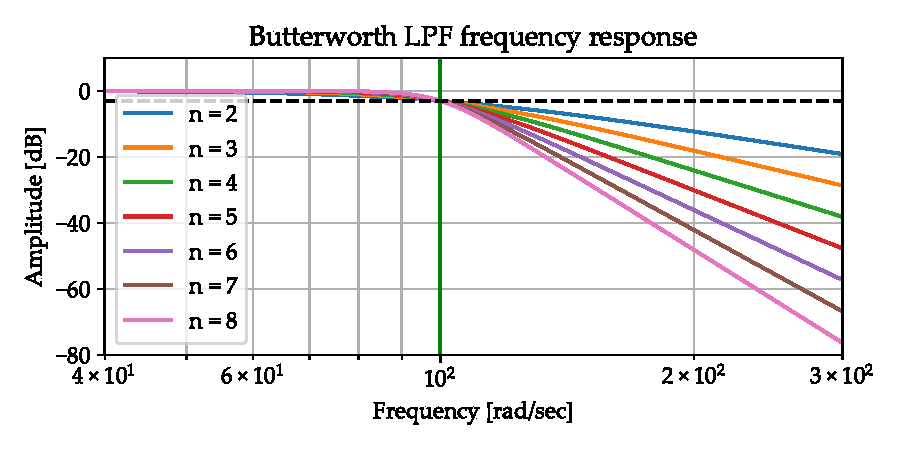
\includegraphics[width=0.45\linewidth]{plots/butterworth-lpf.pdf}
    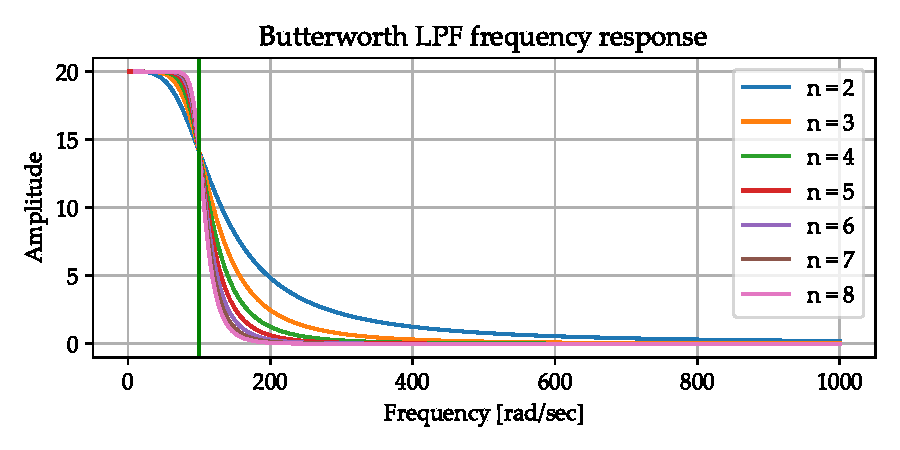
\includegraphics[width=0.45\linewidth]{plots/butterworth-lpf-nolog.pdf}
    \caption{The frequency response of a Butterworth LPF with cut-off frequency $\omega_c = \SI{100}{\radian\per\s}$. The black dash line shows the \SI{-3}{\dB} amplitude.}
    \label{fig:butter-lpf}
\end{figure}
\begin{figure}[htb]
    \centering
    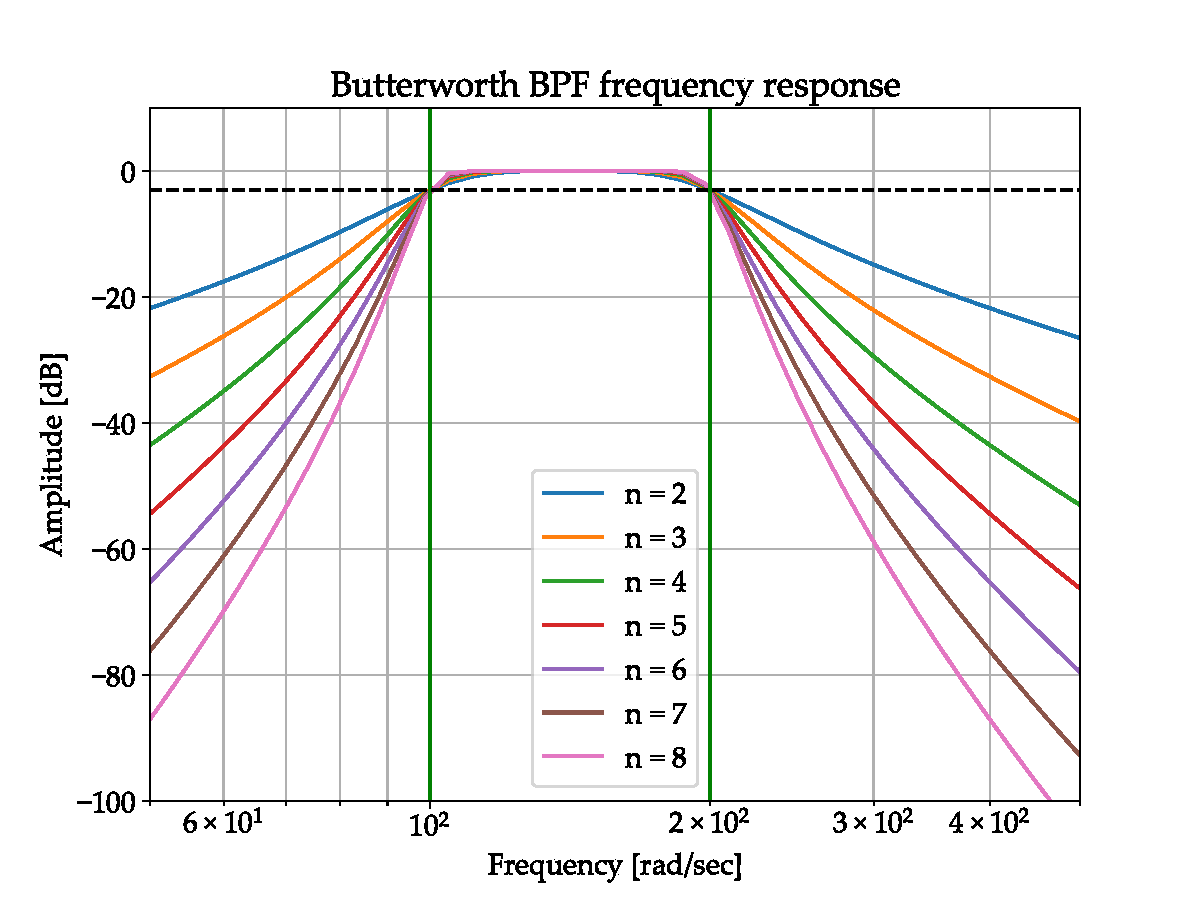
\includegraphics[width=0.45\linewidth]{plots/butterworth-bpf.pdf}
    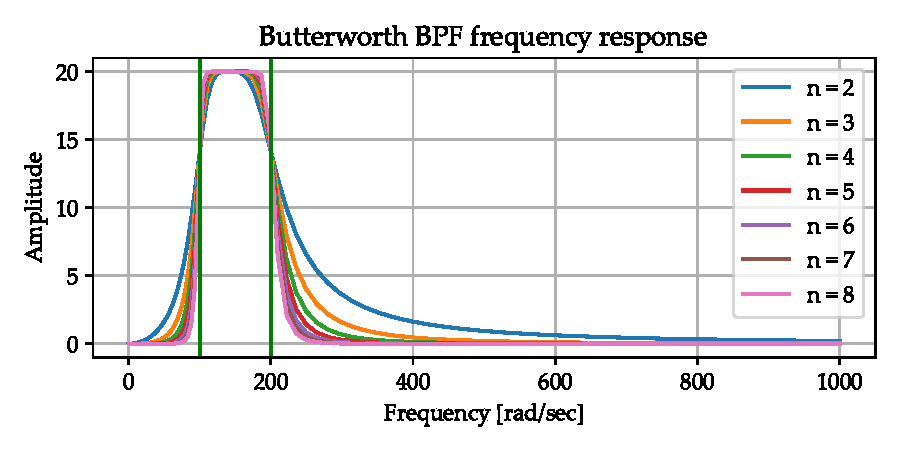
\includegraphics[width=0.45\linewidth]{plots/butterworth-bpf-nolog.pdf}
    \caption{The frequency response of a Butterworth BPF with pass-band from \SI{100}{Hz} to \SI{200}{Hz}. The black dash line shows the \SI{-3}{\dB} amplitude.}
    \label{fig:butter-bpf}
\end{figure}


\section{Additive White Gaussian Noise}
% Definition, principles, and how to generate in Python

\end{document}